\documentclass[conference]{IEEEtran}
\IEEEoverridecommandlockouts
% The preceding line is only needed to identify funding in the first footnote. If that is unneeded, please comment it out.
\usepackage{cite}
\usepackage{amsmath,amssymb,amsfonts}
\usepackage{algorithmic}
\usepackage{graphicx}
\usepackage{textcomp}
\usepackage{xcolor}
\usepackage{pdfpages}

% python shit
% Default fixed font does not support bold face
\DeclareFixedFont{\ttb}{T1}{txtt}{bx}{n}{12} % for bold
\DeclareFixedFont{\ttm}{T1}{txtt}{m}{n}{12}  % for normal

% Custom colors
\usepackage{color}
\definecolor{deepblue}{rgb}{0,0,0.5}
\definecolor{deepred}{rgb}{0.6,0,0}
\definecolor{deepgreen}{rgb}{0,0.5,0}

\usepackage{listings}

% Python style for highlighting
\newcommand\pythonstyle{\lstset{
breaklines=true,
postbreak=\mbox{\textcolor{red}{$\hookrightarrow$}\space},
language=Python,
basicstyle=\ttm,
otherkeywords={self},             % Add keywords here
keywordstyle=\ttb\color{deepblue},
emph={MyClass,__init__},          % Custom highlighting
emphstyle=\ttb\color{deepred},    % Custom highlighting style
stringstyle=\color{deepgreen},
frame=tb,                         % Any extra options here
showstringspaces=false            % 
}}
% Python environment
\lstnewenvironment{python}[1][]
{
\pythonstyle
\lstset{#1}
}
{}

% Python for external files
\newcommand\pythonexternal[2][]{{
\pythonstyle
\lstinputlisting[#1]{#2}}}

% Python for inline
\newcommand\pythoninline[1]{{\pythonstyle\lstinline!#1!}}

\def\BibTeX{{\rm B\kern-.05em{\sc i\kern-.025em b}\kern-.08em
    T\kern-.1667em\lower.7ex\hbox{E}\kern-.125emX}}

\begin{document}

\title{Machine Perception Assignment 2}

\author{\IEEEauthorblockN{Jonathan Wright - 19779085}
\IEEEauthorblockA{\textit{Curtin University} \\
\textit{Computer Science}}}

\maketitle

\begin{abstract}
Within this Assignment I investigated extracting building numbers using various Machine Perception techniques and used
machine learning to interpret those images and make sense of the data.
\end{abstract}

\section{Supervised Learning - Digit Reading}
\subsection{Chosen Classifier}
For this assignment I chose to use a \textbf{Support Vector Machine (SVM)} because in general they perform much faster for this
type of data (low features and low dataset). According to the spec we are more concerned with speed vs accuracy so a drop in
roughly ~5 - 7\% vs using a KNN Classifier is acceptable, hence I chose a SVM.
\subsection{Chosen Feature Set}
I chose to use Hog Feature detection as the OpenCV docs recommended it for OCR, I also considered using SIFT, however, it detects
digits with a 93\% accuracy so I felt no need to switch.

\section{Digit Detection \& Segmentation}
For Digit Detection and Segmentation I have a series of steps, I will list them in order below.
\subsection{Step 1 - Gaussian Blur}
Before I begin trying to extract the images I attempt to blur out as much useless information I can i.e the background,
I found through trial and error optimal values that work for most images to remove almost all useless detected features.
\subsection{Step 2 - Canny Edge Detection}
After blurring the image I use Canny Edge Detection to attempt to detect the edges of the plate or numbers, again through
trial and error I found optimal values that work for most images to remove useless edges.
\subsection{Step 3 - Image Morphological Transformations}
To make certain features more detectable and remove some I used image morphs specifically I first closed the image alot to
make the numbers appear bigger and I also dilated on y more than x to extend them so I could detect them better. Again trial
and error was involved to find optimal values for dilating and closing.
\subsection{Step 4 - Find All Contours In Detected Edges}
Using OpenCV's findContours() method all edges were converted to contours, this will return all the edges areas and x ys.
\subsection{Step 5 - Filtering}
Various filters were used in this step, firstly a area filter is used i.e if the area is too small I disregard it as its
likely not a number. Then I filter by how tall the numbers are or how wide, and I also filter by height width ratio and width
height ratio.
Then after filtering by those I group the contours into pairs, if pairs are found I select these over any other contours.
Finally the contours are returned and this works for all validation images and only 4 training images failed testing.

\section{Performance Of Program}
\subsection{Big O Notation Of Program}
The algorithm I have written I believe is at most O($n^{3}$) where n is the number of contours detected. This is not
what I would call optimal but for this assignment I did not try to optimize the O notation of program as it completes
very quickly already.
\subsection{How Fast The Program Truly Runs (seconds)}
Using Python's inbuilt Time.time() function the program completed training in roughly 0.23 seconds.
It completed validation in roughly 0.16 seconds.
It completed testing in 0.16 seconds (where testing included all validation + training images).
\bfseries{Due to this I can conclude that the program meets the minimum requirement of completing in under one minute.}
\begin{figure}[!htbp]
    \centerline{{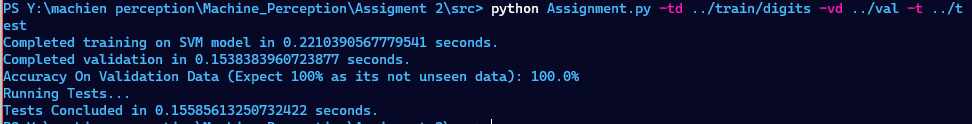
\includegraphics[width=90mm, scale=0.5]{godihatemp.PNG}}}
    \caption{Speed Of Program}
    \label{fig}
\end{figure}

\section{Inspiration or References}
My SVM Model was made following the OpenCV Documentation, other then that I went into this assignment with no inspiration.

\clearpage
\onecolumn
\section{Appendix 1 - Assignment.py}
\pythonexternal{../src/Assignment.py}
\clearpage
\section{Appendix 2 - Training.py}
\pythonexternal{../src/Training.py}
\clearpage
\section{Appendix 3 - Utils.py}
\pythonexternal{../src/Utils.py}
\end{document}
